%  Copyright (C) 2018 by the authors of the World Builder code.
%
%  This file is part of the World Builder.
%
%   This program is free software: you can redistribute it and/or modify
%   it under the terms of the GNU Lesser General Public License as published
%   by the Free Software Foundation, either version 2 of the License, or
%   (at your option) any later version.
%
%   This program is distributed in the hope that it will be useful,
%   but WITHOUT ANY WARRANTY; without even the implied warranty of
%   MERCHANTABILITY or FITNESS FOR A PARTICULAR PURPOSE.  See the
%   GNU Lesser General Public License for more details.
%
%   You should have received a copy of the GNU Lesser General Public License
%   along with this program.  If not, see <https://www.gnu.org/licenses/>.

\documentclass{book} 
\usepackage[utf8]{inputenc}
\usepackage{graphicx}
\usepackage{tikz}
\usepackage{fancyhdr}
\usepackage{titletoc} %needed for chaning the table of contents
%\usepackage{calc}

%\usepackage{makeidx} % Required to make an index
%\makeindex % Tells LaTeX to create the files required for indexing

\graphicspath{{images/}}
\title{World Builder Manual}
\author{menno.fraters }
\date{September 2018}
%%%%%%%%%%%%%%%%%%%%%%%%%%%%%%%%%%%%%%%%%
% The Legrand Orange Book
% Structural Definitions File
% Version 2.0 (9/2/15)
%
% Original author:
% Mathias Legrand (legrand.mathias@gmail.com) with modifications by:
% Vel (vel@latextemplates.com)
% 
% This file has been downloaded from:
% http://www.LaTeXTemplates.com
%
% License:
% CC BY-NC-SA 3.0 (http://creativecommons.org/licenses/by-nc-sa/3.0/)
%
%%%%%%%%%%%%%%%%%%%%%%%%%%%%%%%%%%%%%%%%%

%----------------------------------------------------------------------------------------
%	VARIOUS REQUIRED PACKAGES AND CONFIGURATIONS
%----------------------------------------------------------------------------------------

\usepackage[top=3cm,bottom=3cm,left=3cm,right=3cm,headsep=10pt,a4paper]{geometry} % Page margins

\usepackage{graphicx} % Required for including pictures
\graphicspath{{images/}} % Specifies the directory where pictures are stored

\usepackage{lipsum} % Inserts dummy text

\usepackage{tikz} % Required for drawing custom shapes

\usepackage[english]{babel} % English language/hyphenation

\usepackage{enumitem} % Customize lists
\setlist{nolistsep} % Reduce spacing between bullet points and numbered lists

\usepackage{booktabs} % Required for nicer horizontal rules in tables

\usepackage{xcolor} % Required for specifying colors by name
\definecolor{ocre}{RGB}{0,0,200} % Define the orange color used for highlighting throughout the book

%----------------------------------------------------------------------------------------
%	FONTS
%----------------------------------------------------------------------------------------

\usepackage{avant} % Use the Avantgarde font for headings
%\usepackage{times} % Use the Times font for headings
\usepackage{mathptmx} % Use the Adobe Times Roman as the default text font together with math symbols from the Sym­bol, Chancery and Com­puter Modern fonts

\usepackage{microtype} % Slightly tweak font spacing for aesthetics
\usepackage[utf8]{inputenc} % Required for including letters with accents
\usepackage[T1]{fontenc} % Use 8-bit encoding that has 256 glyphs

%----------------------------------------------------------------------------------------
%	BIBLIOGRAPHY AND INDEX
%----------------------------------------------------------------------------------------
\usepackage{csquotes}
\usepackage[style=numeric,citestyle=numeric,sorting=nyt,sortcites=true,autopunct=true,autolang=hyphen,hyperref=true,abbreviate=false,backref=true,backend=biber]{biblatex}
\addbibresource{bibliography.bib} % BibTeX bibliography file
\defbibheading{bibempty}{}

\usepackage{calc} % For simpler calculation - used for spacing the index letter headings correctly
\usepackage{makeidx} % Required to make an index
\makeindex % Tells LaTeX to create the files required for indexing

%----------------------------------------------------------------------------------------
%	MAIN TABLE OF CONTENTS
%----------------------------------------------------------------------------------------

\usepackage{titletoc} % Required for manipulating the table of contents

\contentsmargin{0cm} % Removes the default margin

% Part text styling
\titlecontents{part}[0cm]
{\addvspace{20pt}\centering\large\bfseries}
{}
{}
{}

% Chapter text styling
\titlecontents{chapter}[1.25cm] % Indentation
{\addvspace{12pt}\large\sffamily\bfseries} % Spacing and font options for chapters
{\color{ocre!60}\contentslabel[\Large\thecontentslabel]{1.25cm}\color{ocre}} % Chapter number
{\color{ocre}}  
{\color{ocre!60}\normalsize\;\titlerule*[.5pc]{.}\;\thecontentspage} % Page number

% Section text styling
\titlecontents{section}[1.25cm] % Indentation
{\addvspace{3pt}\sffamily\bfseries} % Spacing and font options for sections
{\contentslabel[\thecontentslabel]{1.25cm}} % Section number
{}
{\hfill\color{black}\thecontentspage} % Page number
[]

% Subsection text styling
\titlecontents{subsection}[1.25cm] % Indentation
{\addvspace{1pt}\sffamily\small} % Spacing and font options for subsections
{\contentslabel[\thecontentslabel]{1.25cm}} % Subsection number
{}
{\ \titlerule*[.5pc]{.}\;\thecontentspage} % Page number
[]

% List of figures
\titlecontents{figure}[0em]
{\addvspace{-5pt}\sffamily}
{\thecontentslabel\hspace*{1em}}
{}
{\ \titlerule*[.5pc]{.}\;\thecontentspage}
[]

% List of tables
\titlecontents{table}[0em]
{\addvspace{-5pt}\sffamily}
{\thecontentslabel\hspace*{1em}}
{}
{\ \titlerule*[.5pc]{.}\;\thecontentspage}
[]

%----------------------------------------------------------------------------------------
%	MINI TABLE OF CONTENTS IN PART HEADS
%----------------------------------------------------------------------------------------

% Chapter text styling
\titlecontents{lchapter}[0em] % Indenting
{\addvspace{15pt}\large\sffamily\bfseries} % Spacing and font options for chapters
{\color{ocre}\contentslabel[\Large\thecontentslabel]{1.25cm}\color{ocre}} % Chapter number
{}  
{\color{ocre}\normalsize\sffamily\bfseries\;\titlerule*[.5pc]{.}\;\thecontentspage} % Page number

% Section text styling
\titlecontents{lsection}[0em] % Indenting
{\sffamily\small} % Spacing and font options for sections
{\contentslabel[\thecontentslabel]{1.25cm}} % Section number
{}
{}

% Subsection text styling
\titlecontents{lsubsection}[.5em] % Indentation
{\normalfont\footnotesize\sffamily} % Font settings
{}
{}
{}

%----------------------------------------------------------------------------------------
%	PAGE HEADERS
%----------------------------------------------------------------------------------------

\usepackage{fancyhdr} % Required for header and footer configuration

\pagestyle{fancy}
\renewcommand{\chaptermark}[1]{\markboth{\sffamily\normalsize\bfseries\chaptername\ \thechapter.\ #1}{}} % Chapter text font settings
\renewcommand{\sectionmark}[1]{\markright{\sffamily\normalsize\thesection\hspace{5pt}#1}{}} % Section text font settings
\fancyhf{} \fancyhead[LE,RO]{\sffamily\normalsize\thepage} % Font setting for the page number in the header
\fancyhead[LO]{\rightmark} % Print the nearest section name on the left side of odd pages
\fancyhead[RE]{\leftmark} % Print the current chapter name on the right side of even pages
\renewcommand{\headrulewidth}{0.5pt} % Width of the rule under the header
\addtolength{\headheight}{2.5pt} % Increase the spacing around the header slightly
\renewcommand{\footrulewidth}{0pt} % Removes the rule in the footer
\fancypagestyle{plain}{\fancyhead{}\renewcommand{\headrulewidth}{0pt}} % Style for when a plain pagestyle is specified

% Removes the header from odd empty pages at the end of chapters
\makeatletter
\renewcommand{\cleardoublepage}{\newpage}
%\clearpage\ifodd\c@page\else
%\hbox{}
%\vspace*{\fill}
%\thispagestyle{empty}
%\newpage
%\fi}

%----------------------------------------------------------------------------------------
%	THEOREM STYLES
%----------------------------------------------------------------------------------------

\usepackage{amsmath,amsfonts,amssymb,amsthm} % For math equations, theorems, symbols, etc

\newcommand{\intoo}[2]{\mathopen{]}#1\,;#2\mathclose{[}}
\newcommand{\ud}{\mathop{\mathrm{{}d}}\mathopen{}}
\newcommand{\intff}[2]{\mathopen{[}#1\,;#2\mathclose{]}}
\newtheorem{notation}{Notation}[chapter]

% Boxed/framed environments
\newtheoremstyle{ocrenumbox}% % Theorem style name
{0pt}% Space above
{0pt}% Space below
{\normalfont}% % Body font
{}% Indent amount
{\small\bf\sffamily\color{ocre}}% % Theorem head font
{\;}% Punctuation after theorem head
{0.25em}% Space after theorem head
{\small\sffamily\color{ocre}\thmname{#1}\nobreakspace\thmnumber{\@ifnotempty{#1}{}\@upn{#2}}% Theorem text (e.g. Theorem 2.1)
\thmnote{\nobreakspace\the\thm@notefont\sffamily\bfseries\color{black}---\nobreakspace#3.}} % Optional theorem note
\renewcommand{\qedsymbol}{$\blacksquare$}% Optional qed square

\newtheoremstyle{blacknumex}% Theorem style name
{5pt}% Space above
{5pt}% Space below
{\normalfont}% Body font
{} % Indent amount
{\small\bf\sffamily}% Theorem head font
{\;}% Punctuation after theorem head
{0.25em}% Space after theorem head
{\small\sffamily{\tiny\ensuremath{\blacksquare}}\nobreakspace\thmname{#1}\nobreakspace\thmnumber{\@ifnotempty{#1}{}\@upn{#2}}% Theorem text (e.g. Theorem 2.1)
\thmnote{\nobreakspace\the\thm@notefont\sffamily\bfseries---\nobreakspace#3.}}% Optional theorem note

\newtheoremstyle{blacknumbox} % Theorem style name
{0pt}% Space above
{0pt}% Space below
{\normalfont}% Body font
{}% Indent amount
{\small\bf\sffamily}% Theorem head font
{\;}% Punctuation after theorem head
{0.25em}% Space after theorem head
{\small\sffamily\thmname{#1}\nobreakspace\thmnumber{\@ifnotempty{#1}{}\@upn{#2}}% Theorem text (e.g. Theorem 2.1)
\thmnote{\nobreakspace\the\thm@notefont\sffamily\bfseries---\nobreakspace#3.}}% Optional theorem note


\newtheoremstyle{blacknumcodebox} % Theorem style name
{0pt}% Space above
{0pt}% Space below
{\normalfont}% Body font
{}% Indent amount
{\small\bf\sffamily}% Theorem head font
{\;}% Punctuation after theorem head
{0.25em}% Space after theorem head
{\small\sffamily\thmname{#1}\nobreakspace\thmnumber{\@ifnotempty{#1}{}\@upn{#2}}% Theorem text (e.g. Theorem 2.1)
\thmnote{\nobreakspace\the\thm@notefont\sffamily\bfseries---\nobreakspace#3.}\\}% Optional theorem note


% Non-boxed/non-framed environments
\newtheoremstyle{ocrenum}% % Theorem style name
{5pt}% Space above
{5pt}% Space below
{\normalfont}% % Body font
{}% Indent amount
{\small\bf\sffamily\color{ocre}}% % Theorem head font
{\;}% Punctuation after theorem head
{0.25em}% Space after theorem head
{\small\sffamily\color{ocre}\thmname{#1}\nobreakspace\thmnumber{\@ifnotempty{#1}{}\@upn{#2}}% Theorem text (e.g. Theorem 2.1)
\thmnote{\nobreakspace\the\thm@notefont\sffamily\bfseries\color{black}---\nobreakspace#3.}} % Optional theorem note
\renewcommand{\qedsymbol}{$\blacksquare$}% Optional qed square
\makeatother

% Defines the theorem text style for each type of theorem to one of the three styles above
\newcounter{dummy} 
\numberwithin{dummy}{section}
\theoremstyle{ocrenumbox}
\newtheorem{theoremeT}[dummy]{Theorem}
\newtheorem{problem}{Problem}[chapter]
\newtheorem{exerciseT}{Exercise}[chapter]
\theoremstyle{blacknumex}
\newtheorem{exampleT}{Example}[chapter]
\theoremstyle{blacknumbox}
\newtheorem{vocabulary}{Vocabulary}[chapter]
\newtheorem{definitionT}{Definition}[section]
\newtheorem{corollaryT}[dummy]{Corollary}
\theoremstyle{blacknumcodebox}
\newtheorem{codeT}[dummy]{}
\theoremstyle{ocrenum}
\newtheorem{proposition}[dummy]{Proposition}

%----------------------------------------------------------------------------------------
%	DEFINITION OF COLORED BOXES
%----------------------------------------------------------------------------------------

\RequirePackage[framemethod=default]{mdframed} % Required for creating the theorem, definition, exercise and corollary boxes

% Theorem box
\newmdenv[skipabove=7pt,
skipbelow=7pt,
backgroundcolor=black!5,
linecolor=ocre,
innerleftmargin=5pt,
innerrightmargin=5pt,
innertopmargin=5pt,
leftmargin=0cm,
rightmargin=0cm,
innerbottommargin=5pt]{tBox}

% Exercise box	  
\newmdenv[skipabove=7pt,
skipbelow=7pt,
rightline=false,
leftline=true,
topline=false,
bottomline=false,
backgroundcolor=ocre!10,
linecolor=ocre,
innerleftmargin=5pt,
innerrightmargin=5pt,
innertopmargin=5pt,
innerbottommargin=5pt,
leftmargin=0cm,
rightmargin=0cm,
linewidth=4pt]{eBox}	

% Definition box
\newmdenv[skipabove=7pt,
skipbelow=7pt,
rightline=false,
leftline=true,
topline=false,
bottomline=false,
linecolor=ocre,
innerleftmargin=5pt,
innerrightmargin=5pt,
innertopmargin=0pt,
leftmargin=0cm,
rightmargin=0cm,
linewidth=4pt,
innerbottommargin=0pt]{dBox}	

% Corollary box
\newmdenv[skipabove=7pt,
skipbelow=7pt,
rightline=false,
leftline=true,
topline=false,
bottomline=false,
linecolor=gray,
backgroundcolor=black!5,
innerleftmargin=5pt,
innerrightmargin=5pt,
innertopmargin=5pt,
leftmargin=0cm,
rightmargin=0cm,
linewidth=4pt,
innerbottommargin=5pt]{cBox}

% Code box
\newmdenv[skipabove=7pt,
skipbelow=7pt,
backgroundcolor=black!5,
linecolor=ocre,
innerleftmargin=5pt,
innerrightmargin=5pt,
innertopmargin=5pt,
leftmargin=0cm,
rightmargin=0cm,
innerbottommargin=5pt]{codeBox}




% Creates an environment for each type of theorem and assigns it a theorem text style from the "Theorem Styles" section above and a colored box from above
\newenvironment{theorem}{\begin{tBox}\begin{theoremeT}}{\end{theoremeT}\end{tBox}}
\newenvironment{exercise}{\begin{eBox}\begin{exerciseT}}{\hfill{\color{ocre}\tiny\ensuremath{\blacksquare}}\end{exerciseT}\end{eBox}}				  
\newenvironment{definition}{\begin{dBox}\begin{definitionT}}{\end{definitionT}\end{dBox}}	
\newenvironment{example}{\begin{exampleT}}{\hfill{\tiny\ensuremath{\blacksquare}}\end{exampleT}}		
\newenvironment{corollary}{\begin{cBox}\begin{corollaryT}}{\end{corollaryT}\end{cBox}}	
\usepackage{listings}
\usepackage[most]{tcolorbox}
\usepackage{inconsolata}
\usepackage{accsupp} % for having non-copyable line numbers
\usepackage{tabularx}

\definecolor{mygreen}{rgb}{0.1,0.8,0.1}

\definecolor{mygray}{rgb}{0.5,0.5,0.5}
\definecolor{lightgray}{rgb}{0.8,0.8,0.8}

\newcommand\emptyaccsupp[1]{\BeginAccSupp{ActualText={}}#1\EndAccSupp{}}

\newtcblisting[auto counter]{bashcode}[2][]{sharp corners, 
    fonttitle=\bfseries, colframe=ocre!60, listing only, top=0pt, bottom=0pt, left=20pt, lefttitle=0pt,
    listing options={basicstyle=\ttfamily,language=bash, commentstyle=\color{mygreen}, numberstyle=\small\emptyaccsupp\bf\color{mygray}, columns=flexible, numbers=left, stepnumber=1, showspaces=false, showstringspaces=false}, before=\vspace{10pt}\noindent, after=\vspace{10pt}, title=Listing \thetcbcounter: #2, #1}
    
\newtcblisting[auto counter]{fortrancode}[2][]{sharp corners, 
    fonttitle=\bfseries, colframe=ocre!60, listing only, top=0pt, bottom=0pt, left=20pt, lefttitle=0pt,
    listing options={basicstyle=\ttfamily,language=fortran, commentstyle=\color{mygreen}, numberstyle=\small\emptyaccsupp\bf\color{mygray}, columns=flexible, numbers=left, stepnumber=1, showspaces=false, showstringspaces=false}, before=\vspace{10pt}\noindent, after=\vspace{10pt},
    title=Listing \thetcbcounter: #2, #1}
    
%    \newtcblisting[auto counter]{parameterbox}[4][]{sharp corners, 
%    fonttitle=\bfseries, colframe=ocre!60, listing only, top=0pt, bottom=0pt, left=0pt, lefttitle=0pt,
%    listing options={showspaces=false, showstringspaces=false, breaklines=true}, 
%    title=Parameter \thetcbcounter: name: #2 -- required: #3 -- type: #4, #1}
 \newenvironment{parameterbox}[4]{\begin{tcolorbox}[title={ \begin{tabularx}{\textwidth}{ l  | X | l | X }Name: #1 & Required: #2 & Type: #3 & Default: #4\end{tabularx}},colframe=ocre!60]}{  \end{tcolorbox}}
    \usepackage{color,soul} %for highlighting text
    \sethlcolor{lightgray}
    %\newcommand{\hlc}[2][yellow]{ {\sethlcolor{#1} \hl{#2}} }
    
%\newenvironment{code}{\begin{codeBox}\begin{codeT}}{\end{codeT}\end{codeBox}}	

\usepackage{titlesec}

\setcounter{secnumdepth}{4}

\titleformat{\paragraph}
{\normalfont\normalsize\bfseries}{\theparagraph}{1em}{}
\titlespacing*{\paragraph}
{0pt}{3.25ex plus 1ex minus .2ex}{1.5ex plus .2ex}

%----------------------------------------------------------------------------------------
%	REMARK ENVIRONMENT
%----------------------------------------------------------------------------------------

\newenvironment{remark}{\par\vspace{10pt}\small % Vertical white space above the remark and smaller font size
\begin{samepage}\begin{list}{}{
\leftmargin=35pt % Indentation on the left
\rightmargin=25pt}\item\ignorespaces % Indentation on the right
\makebox[-2.5pt]{\begin{tikzpicture}[overlay]
\node[draw=ocre!60,line width=1pt,circle,fill=ocre!25,font=\sffamily\bfseries,inner sep=2pt,outer sep=0pt] at (-15pt,0pt){\textcolor{ocre}{R}};\end{tikzpicture}} % Orange R in a circle
\advance\baselineskip -1pt}{\end{list}\end{samepage}\vskip5pt} % Tighter line spacing and white space after remark

%----------------------------------------------------------------------------------------
%	SECTION NUMBERING IN THE MARGIN
%----------------------------------------------------------------------------------------

\makeatletter
\renewcommand{\@seccntformat}[1]{\llap{\textcolor{ocre}{\csname the#1\endcsname}\hspace{1em}}}                    
\renewcommand{\section}{\@startsection{section}{1}{\z@}
{-4ex \@plus -1ex \@minus -.4ex}
{1ex \@plus.2ex }
{\normalfont\large\sffamily\bfseries}}
\renewcommand{\subsection}{\@startsection {subsection}{2}{\z@}
{-3ex \@plus -0.1ex \@minus -.4ex}
{0.5ex \@plus.2ex }
{\normalfont\sffamily\bfseries}}
\renewcommand{\subsubsection}{\@startsection {subsubsection}{3}{\z@}
{-2ex \@plus -0.1ex \@minus -.2ex}
{.2ex \@plus.2ex }
{\normalfont\small\sffamily\bfseries}}                        
\renewcommand\paragraph{\@startsection{paragraph}{4}{\z@}
{-2ex \@plus-.2ex \@minus .2ex}
{.1ex}
{\normalfont\small\sffamily\bfseries}}

%----------------------------------------------------------------------------------------
%	PART HEADINGS
%----------------------------------------------------------------------------------------

% numbered part in the table of contents
\newcommand{\@mypartnumtocformat}[2]{%
\setlength\fboxsep{0pt}%
\noindent\colorbox{ocre!20}{\strut\parbox[c][.7cm]{\ecart}{\color{ocre!70}\Large\sffamily\bfseries\centering#1}}\hskip\esp\colorbox{ocre!40}{\strut\parbox[c][.7cm]{\linewidth-\ecart-\esp}{\Large\sffamily\centering#2}}}%
%%%%%%%%%%%%%%%%%%%%%%%%%%%%%%%%%%
% unnumbered part in the table of contents
\newcommand{\@myparttocformat}[1]{%
\setlength\fboxsep{0pt}%
\noindent\colorbox{ocre!40}{\strut\parbox[c][.7cm]{\linewidth}{\Large\sffamily\centering#1}}}%
%%%%%%%%%%%%%%%%%%%%%%%%%%%%%%%%%%
\newlength\esp
\setlength\esp{4pt}
\newlength\ecart
\setlength\ecart{1.2cm-\esp}
\newcommand{\thepartimage}{}%
\newcommand{\partimage}[1]{\renewcommand{\thepartimage}{#1}}%
\def\@part[#1]#2{%
\ifnum \c@secnumdepth >-2\relax%
\refstepcounter{part}%
\addcontentsline{toc}{part}{\texorpdfstring{\protect\@mypartnumtocformat{\thepart}{#1}}{\partname~\thepart\ ---\ #1}}
\else%
\addcontentsline{toc}{part}{\texorpdfstring{\protect\@myparttocformat{#1}}{#1}}%
\fi%
\startcontents%
\markboth{}{}%
{\thispagestyle{empty}%
\begin{tikzpicture}[remember picture,overlay]%
\node at (current page.north west){\begin{tikzpicture}[remember picture,overlay]%	
\fill[ocre!20](0cm,0cm) rectangle (\paperwidth,-\paperheight);
\node[anchor=north] at (4cm,-3.25cm){\color{ocre!40}\fontsize{220}{100}\sffamily\bfseries\thepart}; 
\node[anchor=south east] at (\paperwidth-1cm,-\paperheight+1cm){\parbox[t][][t]{8.5cm}{
\printcontents{l}{0}{\setcounter{tocdepth}{1}}%
}};
\node[anchor=north east] at (\paperwidth-1.5cm,-3.25cm){\parbox[t][][t]{15cm}{\strut\raggedleft\color{white}\fontsize{30}{30}\sffamily\bfseries#2}};
\end{tikzpicture}};
\end{tikzpicture}}%
\@endpart}
\def\@spart#1{%
\startcontents%
\phantomsection
{\thispagestyle{empty}%
\begin{tikzpicture}[remember picture,overlay]%
\node at (current page.north west){\begin{tikzpicture}[remember picture,overlay]%	
\fill[ocre!20](0cm,0cm) rectangle (\paperwidth,-\paperheight);
\node[anchor=north east] at (\paperwidth-1.5cm,-3.25cm){\parbox[t][][t]{15cm}{\strut\raggedleft\color{white}\fontsize{30}{30}\sffamily\bfseries#1}};
\end{tikzpicture}};
\end{tikzpicture}}
\addcontentsline{toc}{part}{\texorpdfstring{%
\setlength\fboxsep{0pt}%
\noindent\protect\colorbox{ocre!40}{\strut\protect\parbox[c][.7cm]{\linewidth}{\Large\sffamily\protect\centering #1\quad\mbox{}}}}{#1}}%
\@endpart}
\def\@endpart{\vfil\newpage
\if@twoside
\if@openright
%\null
%\thispagestyle{empty}%
%\newpage
\fi
\fi
\if@tempswa
\twocolumn
\fi}

%----------------------------------------------------------------------------------------
%	CHAPTER HEADINGS
%----------------------------------------------------------------------------------------

% A switch to conditionally include a picture, implemented by  Christian Hupfer
\newif\ifusechapterimage
\usechapterimagetrue
\newcommand{\thechapterimage}{}%
\newcommand{\chapterimage}[1]{\ifusechapterimage\renewcommand{\thechapterimage}{#1}\fi}%
\newcommand{\autodot}{.}
\def\@makechapterhead#1{%
{\parindent \z@ \raggedright \normalfont
\ifnum \c@secnumdepth >\m@ne
\if@mainmatter
\begin{tikzpicture}[remember picture,overlay]
\node at (current page.north west)
{\begin{tikzpicture}[remember picture,overlay]
\node[anchor=north west,inner sep=0pt] at (0,0) {\ifusechapterimage\includegraphics[width=\paperwidth]{\thechapterimage}\fi};
\draw[anchor=west] (\Gm@lmargin,-2.5cm) node [line width=2pt,rounded corners=15pt,draw=ocre,fill=white,fill opacity=0.5,inner sep=15pt]{\strut\makebox[22cm]{}};
\draw[anchor=west] (\Gm@lmargin+.3cm,-2.5cm) node {\huge\sffamily\bfseries\color{black}\thechapter\autodot~#1\strut};
\end{tikzpicture}};
\end{tikzpicture}
\else
\begin{tikzpicture}[remember picture,overlay]
\node at (current page.north west)
{\begin{tikzpicture}[remember picture,overlay]
\node[anchor=north west,inner sep=0pt] at (0,0) {\ifusechapterimage\includegraphics[width=\paperwidth]{\thechapterimage}\fi};
\draw[anchor=west] (\Gm@lmargin,-2.5cm) node [line width=2pt,rounded corners=15pt,draw=ocre,fill=white,fill opacity=0.5,inner sep=15pt]{\strut\makebox[22cm]{}};
\draw[anchor=west] (\Gm@lmargin+.3cm,-2.5cm) node {\huge\sffamily\bfseries\color{black}#1\strut};
\end{tikzpicture}};
\end{tikzpicture}
\fi\fi\par\vspace*{20\p@}}}

%-------------------------------------------

\def\@makeschapterhead#1{%
\begin{tikzpicture}[remember picture,overlay]
\node at (current page.north west)
{\begin{tikzpicture}[remember picture,overlay]
\node[anchor=north west,inner sep=0pt] at (0,0) {\ifusechapterimage\includegraphics[width=\paperwidth]{\thechapterimage}\fi};
\draw[anchor=west] (\Gm@lmargin,-2.5cm) node [line width=2pt,rounded corners=15pt,draw=ocre,fill=white,fill opacity=0.5,inner sep=15pt]{\strut\makebox[22cm]{}};
\draw[anchor=west] (\Gm@lmargin+.3cm,-2.5cm) node {\huge\sffamily\bfseries\color{black}#1\strut};
\end{tikzpicture}};
\end{tikzpicture}
\par\vspace*{20\p@}}
\makeatother

%----------------------------------------------------------------------------------------
%	HYPERLINKS IN THE DOCUMENTS
%----------------------------------------------------------------------------------------

\usepackage{hyperref}
\hypersetup{hidelinks,colorlinks=false,breaklinks=true,urlcolor= ocre,bookmarksopen=false,pdftitle={The Geodynamic World Builder Manual},pdfauthor={The Geodynamic World Builder}}
\usepackage{bookmark}
\bookmarksetup{
open,
numbered,
addtohook={%
\ifnum\bookmarkget{level}=0 % chapter
\bookmarksetup{bold}%
\fi
\ifnum\bookmarkget{level}=-1 % part
\bookmarksetup{color=ocre,bold}%
\fi
}
}


\newcommand{\GWB}{{Geodynamic World Builder}}
\newcommand{\WB}{{World Builder}}
\newcommand{\paraview}{{Paraview}}
\newcommand{\boost}{{Boost}}
\newcommand{\ghost}{{GHOST}}
\newcommand{\aspect}{{ASPECT}}
\newcommand{\elephant}{{EleFhant}}
\newcommand{\cmake}{{cmake}}
\newcommand{\gcov}{{Gcov}}

\begin{document}
\usechapterimagefalse
\begingroup
\thispagestyle{empty}
\begin{tikzpicture}[remember picture,overlay]
\node[inner sep=0pt] (background) at (current page.center) {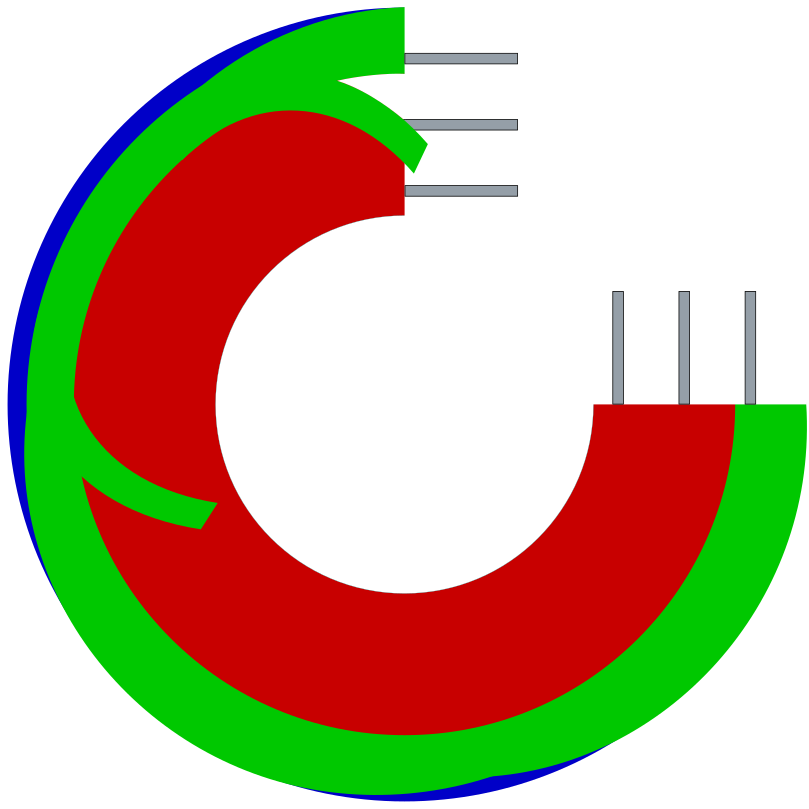
\includegraphics[width=\paperwidth]{world_builder_logo_v4.png}};
\draw (current page.center) node [fill opacity=0.0,text opacity=1,inner sep=1cm]{\Huge\centering\bfseries\sffamily\parbox[c][][t]{\paperwidth}{\centering  Manual of \\  the Geodynamic \\ World Builder \\ [10pt] 
{\Large geodynamicworldbuilder.github.io} \\ [10pt] {\huge version 0.1.0-pre}}}; 
\draw (current page.south) node [fill opacity=0.0,text opacity=1,inner sep=1cm]{\Large\centering\bfseries\sffamily\parbox[t][][t]{\paperwidth}{\centering  Written by Menno Fraters \\ [100pt]}}; 
\end{tikzpicture}
\vfill
\endgroup
%\newpage
%\pagestyle{empty} % No headers

\tableofcontents
%\cleardoublepage
\pagestyle{fancy}




\part{An overview of the Geodynamic World builder}
\chapter{Introduction}
The \GWB{} (\url{https://geodynamicworldbuilder.github.io}), or in short \WB{}, is a code library intended to set up initial conditions for computational geodynamic models in both Cartesian and Spherical coordinates. This means that it can provide properties like temperature and how much of what composition or material is where in the model. It uses a JSON style parameter file to set up a mathematical representation of the world, which can then be sampled. The input for the JSON style parameter file are not complex equations, but a structured form to describe tectonic features. This can be for example a continental plate, an oceanic plate or a subducting plate. Each of these tectonic features can be assigned a specific model representing its temperature or composition. In short, this software has been designed to for a bridge between plate tectonic interpretation and geodynamic modelling.
\\
The \WB{} is a c++ stand alone library, which only has a dependency on the \boost{} library (\url{https://boost.org}), and has wrappers for both c and fortran available. Besides this library, the \WB{} repository also contains two utility programs. The first one is the app. This program is a command line application which allows a user or an other program to use the \WB{} library directly from the command line. The second program is the \WB{} Visualization program. This program allows users to visualize their models through \paraview{} (\url{https://paraview.org}) files. This code is based on \ghost{} \cite{Thieulot_2018}, which is available at \url{https://github.com/cedrict/GHOST}. The \WB{} has already been successfully used in both the c++ FEM \aspect{} \cite{KHB12,heister_aspect_methods2,aspect-doi-v2.0.1,aspectmanual} and the fortran FEM \elephant{} \cite{Thieulot_2017}.
\section{The idea behind the World Builder}
\label{section:idea_behind_WB}
In geodynamic modelling, setting up a simple complexity model is, not surprisingly, easy. Setting up a very complex model, based on data such as tomography is also reasonably simple, ignoring all kind of complex conversions usually needed, because one just has to load in the data. But setting up models of intermediary complexity, e.g. models which are synthetic but try to resemble an actual location on the earth, is very hard. This has to do with the fact that simple models are usually set up with a simple equation and a few if/else statements. In two dimensions, this is usually still manageable, although even here the equations involved quickly become unmanageable. With the advance of the availability of more powerful computer to the geodynamic community, regional 3d problems come within computational range. But this also exponentially increases the problem with the setting up complex synthetic models. Although it is not impossible to set up such complex synthetic models in 3d, implementing it in an naive way will result in code which is extremely hard to read, even for the authors themselves and nearly impossible to maintain. Furthermore, using such approaches makes it nearly impossible to read and modify for both students and non-model development experts, who want to set up a model for their geological or geodynamic problem. 
\\ 
An other problem with these intermediary complexity models is that they are very hard to exactly reproduce in other models. This because geodynamic models do not all support the same kind of features when it comes to setting up for example temperature and composition. 
\\
The \GWB{} hopes to solve these, and some other, problems, by implementing the following design principles:
\\
\begin{enumerate}
    \item {\bf Design input around plate tectonics:} Have an input file, which is at its core a text based file, where users can enter the plate tectonic features they would like to model by name, and where they should be place in the world. For each plate tectonic feature, they should be able to select for every property a specific module to model that property in the way they want. Depending on the model, they might be asked to provide some information to specify what the model should repesent exactly. For example, they may want to define an oceanic plate at a certain position, and set its temperature model to a half-space cooling model. In this example they will be asked to provide the coordinate points of the ridge, the spreading velocity and to what depth this model should be active. They will also be able to name all the different features, so that it is clear what each feature represents.
    \item {\bf Code and language independent:} There are many different codes to model geodyamic problems, for which many different languages are used. The \WB{} is designed to be easy to integrate in these codes. Although the library itself is written in c++, it has an official c and fortran interface and it is possible to call it from the command line. Trough the c wrapper it is also possible to call the \WB{} from almost any other language like phyton and mathlab. 
    \item {\bf Reproducibility: } In science it is very important to be able to repeat experiments to test their validity. Although there are more challenges with reproducability of model than just initial conditions, it is one of the important ones. It is therefore crucial that a single \WB{} input file, should always yield the same output. On the other hand, it is important to able to fix problem when they are found, or use new insights into ways to better organize the input. We have a two track approach to this problem:
    \begin{itemize}
        \item {\bf Documentation: } The \WB{} is generating models. And models will never be exactly the same as reality. That means that there are approximation used in creating these models. As long as the person who uses the \WB{} to design their model is aware of what the \WB{} does, and what approximation it uses, that person can make an informed decision whether those approximations are dependable in their application. It is therefore important to not only document how to use a function, but also explain what approximations are used and the code does. 
        \item {\bf Version numbering: } When a problem can't be solved in a backwards compatible way, we will make use of the version system. To this end we use Semantic Versioning 2.0.0 (\url{https://semver.org/spec/v2.0.0.html}). This means that from version 1.0.0, every change to the code which is backwards incompatible with the input file or the interface we provide, we will increase the major version. We require every \WB{} input file to contain the current major version number. This way it is always clear what version of the code was used to produce the model.
    \end{itemize}
    \item {\bf Safe use in parallel codes:} The \WB{} is designed for large problems, and should therefore be safe to use in parallel codes. This means that the library itself is split into two parts, a setup phase in which both reading and writing in global persistent variables is allowed, and a using phase, in which only reading from these variables is allowed. The first phase is encapsulated in the function which creates the world. When this function is done (which may be done per MPI process or one time globally and then shared), the world object is thread-safe to query the temperature and composition at different locations.
    \item {\bf Readable and extendable code:} Making model modules, or even tectonic features for all possible initial conditions which are used and will be used in the community is a big and continuously changing task. Following the example of \aspect{} we have implemented a plugin system for different parts of the code. This allows beginning developers to only focus on understanding the code they are interested in, without having to worry too much about what the rest of the code is doing. 
\end{enumerate}

\section{Citing the world builder}
The \GWB{} is currently not published yet, so it can't be cited. Please check back later.
\section{Acknowledgments}
The development of the \GWB{} has through the author been supported by NWO, CEED and CIG? And thank the ASPECT community for their support?



\chapter{Installation}
\section{Installation requirements and dependencies}
\label{section:dependencies}
The world builder is currently only official supports Linux operating systems, although it should be possible to work with OSX and Windows. The only requirement are a c++ compiler with at minimum c++11 is installed together with the boost library (\url{https://boost.org}), \cmake{} (\url{https://cmake.org/}) and gfortran. 


\section{What is in the package?}
\label{section:in_package}
When the \GWB{} is downloaded, it contains the main library, two programs and a tester package. Each one is described in more detail in the next few sections.
\subsection{The World Builder library}
This is the main code of the \GWB{}. In this library all the code relating to setting up and querying the \WB{} world. It also contains the wrapper code to interface from c and fortran programs. This part is dependent on the \boost{} property tree. 

\subsection{The World Builder app}
This is a program which can be used to query the \WB{} from the command line, by providing it a world builder file, and then a data file. This data file should contain in the header information on the dimension you want to use and the amount of compositions, and in the main part the required information like for example for a 3d case x,y and z position, depth and gravity (See Listing \ref{lst:code_example_app_input_data_file}). The output of the data file from listing \ref{lst:code_example_app_input_data_file},, with a certain \WB{} file, is presented in Listing \ref{lst:code_example_app_out}. This program is dependent on \boost{} program options.

\begin{bashcode}[label={lst:code_example_app_input_data_file}]{Example input data file}
# This is a comment in the data
# file. 
# Now define parameters:
# dim = 2
# compositions = 5
# x      z d g  T c1 c2 c3 c4 c5
  1      2 2 10
  2      2 2 10
  3      4 0 10
  560e3  0 0 10
  1999e3 0 0 10
\end{bashcode}

\begin{bashcode}[label={lst:code_example_app_out}]{Example output from above input for the \WB{} app}
# x z d T c0 c1 c2 c3 c4 
1 2 2 10 1600 0 0 0 0 0 
2 2 2 10 1600 0 0 0 0 0 
3 4 0 10 1600 0 0 0 0 0 
560e3 0 0 10 150 0 0 0 1 0 
2000e3 0 0 10 20 0 0 1 0 0
\end{bashcode}

\subsection{The World Builder Visualization program}
This program helps with visualizing the \WB{} file by producing pvd files which can be opened with visualization programs like \paraview{}. It requires a \WB{} file and a grid file to be provided. A grid file is a special format file which contains information about what part of the \WB{} domain should be visualized. An example of a grid file can be found in Listing \ref{lst:code_example_grid_file}.

\begin{bashcode}[label={lst:code_example_grid_file}]{An example of a grid file for a 3d cartesian grid.}
# ouput variables
grid_type = cartesian
dim = 3
compositions = 2

# domain of the grid
x_min = 0e3
x_max = 2000e3
y_min = 0e3
y_max = 1000e3
z_min = 0 
z_max = 750e3

# grid properties
n_cell_x = 160
n_cell_y = 80
n_cell_z = 60
\end{bashcode}

\subsection{The tester}
It is important for every software to be propery tested. The \WB{} is no exception. We currently have two types of test implemented. The first, and currently the most important one, is the unit tester. This tester allows to test individual function functions of the \WB{} library in relative isolation. The second type of tester is an integration tester, which works through the \WB{} app. This tester tests whether the whole library works in the expected way it is supposed to by providing a \WB{} file and data points to get temperature and composition from them. The tester is run ever time on proposed new code before that code is added to the main \WB{} repository, and all test have to pass before it can be merged. This happens through Travis CI (see \url{https://travis-ci.org/GeodynamicWorldBuilder/WorldBuilder}).

\subsubsection{Tester coverage}
Having tests alone is not good enough to make sure that the actually does what it is supposed to do. The tester should theoretically cover all the possible cases which a software package can provide. In practice we test the coverage by counting the number of 'relevant' lines and how much of these lines are touched when running the tester. This is counted and reported by the program \gcov{} (\url{https://gcc.gnu.org/onlinedocs/gcc/Gcov.html}).
\\
This approach is not perfect and has two main problems. The first problem is that a 100\% coverage is practically not achievable, since it code might have have assertions in places which should never be reached. The second problem is that even though a line of code is touched by the tester, it may not mean that all possible cases in that line are tested. Think for example of an inline if statement, or an assertion macro line. These lines count as being touched by the tester, but only one case may actually be tested.
\\
As long as these limits are kept in mind, there is no problem in using this kind of coverage to test the tester quality. Keeping these limits in mind, we try to keep the code above 95\% coverage. At the time of writing the coverage is above 97.5\%. The coverage is measured and reported every time when new code is proposed. This happens through Coveralls (see \url{https://coveralls.io/github/GeodynamicWorldBuilder/WorldBuilder}).


\section{Installation guidelines for different cases}
When installing the \WB{} on a Linux system, make sure \cmake{}, \boost{} with  program options and gfortran are installed. This can be done through the command: \hl{apt install cmake gfortran libboost libboost-program-options-dev}.
\begin{remark}
See Section \ref{section:dependencies} for more details the minimum requirements of the \WB{}.
\end{remark}

\subsection{Installing it as a stand alone program}
\label{subsection:install_stand_aline}
\begin{enumerate}
    \item Make a directory where you want to install it to (e.g. \hl{mkdir world\_builder}).
    \item Enter that directory (e.g. \hl{cd world\_builder}).
    \item clone the git repository from github (e.g. \hl{git clone  \\ \hbox{\url{ git@github.com:GeodynamicWorldBuilder/WorldBuilder.git}}}). Make sure you have a working github account.
    \item enter the new world builder directory (e.g. \hl{cd WorldBuilder}).
    \item make a build directory and enter it.
    \item run cmake by entering: \hl{cmake ..}.
    \item make sure cmake finds all the dependencies.
    \item run make with the ammount of thread you want to use (e.g. use 8 processes: \hl{make -j 8}).
    \item run the tests to make sure everything installed correctly (\hl{ctest}).
\end{enumerate}
Now all the library, tester and the two programs, described in section \ref{section:in_package}, are ready for use.

\subsection{Installing it as part of a cpp program}
For this case, there are two options. Either compile the library and link it, or directly compile the library source files within your project.

\subsubsection{Compile the library and link it}
First follow the instructions from section \ref{subsection:install_stand_aline}. The library can be found in the \hl{build/lib/} directory with the name \hl{libWorldBuilder.a}. Link your project with this file. 
\\
The only file you need to include in your code is \hl{world\_builder/world.h}. Initialize a variable of type \hl{WorldBuilder::World} with a valid std::string pointing to the world builder file. Then implement in the correct locations the temperature and composition querying functions.

\subsubsection{Directly compile the library source files within your project}
\label{subsubsection:direct_compile_library_source}
This is the way it is implemented in \aspect{}. Although it is possible to just copy the library sourc and head directory files, it is recommended to clone the whole world builder project into a directory in your project (possibly as a git submodule). This way the \WB{} can be easily updated. Add the \WB{} files to cmake/make/compiler. 
\\
The only file you need to include in your code is \hl{world\_builder/world.h}. Initialize a variable of type \hl{WorldBuilder::World} with a valid std::string pointing to the world builder file. Then implement in the correct locations the temperature and composition querying functions.
\subsection{Installing it as part of a c program}
First follow the instructions from section \ref{subsection:install_stand_aline}.The library can be found in the \hl{build/lib/} directory with the name \hl{libWorldBuilder.a}. Link your project with this file. 
\\
The only file you need to include in your code is \hl{world\_builder/wrapper\_c.h}. Create a void variable which is a pointer to a pointer and set it so NULL (e.g. \hl{void **ptr\_ptr\_world}), and create a pointer to a c-string (e.g. \hl{char *world\_builder\_file}). Pass these variables to the \hl{create\_world} function. This function will create the \WB{} world. Now this pointer can be used to call the temperture and composition quering functions. When done with the \WB{}, call the \hl{release\_world} function. This will clean up the memory used by the world builder.
\begin{remark}
Do not forget to call release\_world, when done with the \WB{}.
\end{remark}

\subsection{Installing it as part of a fortran program}
First follow the instructions from section \ref{subsection:install_stand_aline}.The library can be found in the \hl{build/mod/} directory with the name \hl{worldbuilder.mod}. Link your project with this file. 
\\
Include the module into your project. The only thing you need to care for, when creating the world is to provide file name which ends with \hl{//C\_NULL\_CHAR}. Then call the \hl{create\_world} function with the variable \hl{cworld} and the file name variable. The fortran module takes care of the world pointer internally. When the \WB{} world is created, the temperature and composition functions can be called at will. When done with the \WB{} call the function \hl{release\_world(cworld)}. 
\begin{remark}
Do not forget to call release\_world, when done with the \WB{}.
\end{remark}
To be more clear, we show here an example fortran program using the \GWB{}. 

\begin{fortrancode}{Example how to interface the \WB{} with fortran code}
program test
use WorldBuilder

IMPLICIT NONE

  ! Declare the types which will be needed.
  REAL*8 :: temperature,x=120e3,y=500e3,z=0,depth=0,gravity = 10
  INTEGER :: composition_number = 3
  REAL*8 :: composition
  character(len=256) :: file_name = "path/to/world_builder_file"//C_NULL_CHAR

  ! Show how to call the functions.
  CALL create_world(cworld, file_name)

  write(*, *) '2d temperature:'
  CALL temperature_2d(cworld,x,z,depth,gravity,temperature)
  write(*, *) 'temperature in fortran = ', temperature

  write(*, *) '3d temperature:'
  CALL temperature_3d(cworld,x,y,z,depth,gravity,temperature)
  write(*, *) 'temperature in fortran = ', temperature

    write(*, *) '2d composition:'
  CALL composition_2d(cworld,x,z,depth,composition_number,composition)
  write(*, *) 'composition in fortran = ', composition

  write(*, *) '3d composition:'
  CALL composition_3d(cworld,x,y,z,depth,composition_number,composition)
  write(*, *) 'composition in fortran = ', composition

  CALL release_world(cworld)
END program
\end{fortrancode}

A more extinsive example for how to link fortran code with the \WB{} can be found in the example directory. This includes instructions on how to compile the example.

\subsection{Installing it as part of ASPECT}
The \GWB{} is currently implemented in \aspect{} as a submodule, with a method similar to what is described in section \ref{subsubsection:direct_compile_library_source}, where ASPECT can be directly compiled with the \WB{} source files. The only thing you have to do, is to make sure that the submodule is actually loaded.
\\
 If the \WB{} submodule is initialized, \aspect{}'s \cmake{} configuration will automatically find it and use it. When cloning the \aspect{} repository, add the \hl{--recursive} flag, to automatically initialize the git submodule. If you already cloned \aspect{}, use the command \hl{git submodule update --init --recursive}. 
 \\
 When \aspect{} as been successfully compiled with the \WB{}, set the \aspect{} global input parameter \hl{World builder file} to the \WB{} file location. 


\chapter{Using the World builder}
\section{Introduction}
When the \WB{} is installed and coupled correctly to the geodynamics code of your choosing, you will only need to create the correct \WB{} file for your problem. This section of the manual will explain how the \WB{} file is designed, and how it can be used to create complex problems in both 2d and 3d. 
\section{Design of the \WB{} input file}
\subsection{JSON}
One of the goals of the \GWB{} is to make it easy for users to create very complex initial conditions, with only providing the most essential information needed to create that complex initial condition. To be more concrete, we want users to just fill in data on how they want their model to look like, and the \WB{} should do the rest. For this reason we have chosen the data file format JSON to form the basis of the \WB{} file. It is designed to have data in a format which is readable and writable by both humans and computers, which is what is the intent of this file. 
\begin{remark}
There are also some downsides to using a JSON based format, one of which is that is doesn't support comments directly in the file. It is possible to add a comment value in any field, which will be ignored by the \WB{}.
\end{remark}
\subsection{A minimum world builder example}
To understand how the \WB{} file is structured, let's begin with a minimal example. The only things which are always required in the file are a value called \hl{version} and a object called \hl{Surface ojbects}:

\begin{bashcode}{A minimal \WB{} example}
"version":0,
"surface objects":{}
\end{bashcode}

This example obviously doesn't do much. Yet a lot is already happening in the background. To make life easy, parameters can be set to default values, which also the case here. The version number indicates the major version number of the \GWB{}. Because we follow the Semantic Versioning 2.0.0 (\url{https://semver.org/spec/v2.0.0.html}) guidlines, every time (after the release of version 1.0.0) there is no other way than making changes to the \WB{} which would change the result given the same input file, the major version number is increased. After the release of version 1.0.0 of the \GWB{}, we will do our best to keep backwards compatibility as long as possible.
\\
If you where to visualize the temperature and the compositions of this model, you would see an adiabatic temperature profile and all compositions returning zero. One of the most important of the global parameters which has a default value is the coordinate system. More on that later, for now here is an example which shows what that parameter looks like:

\begin{bashcode}[label={lst:code_minimal_example_default_coordinate_system}]{A minimal example explicitly showing the default coordinate system}
"version":0,
"coordinate system":{"cartesian":{}},
"surface objects":{}
\end{bashcode}

This already shows some interesting features of the JSON file. First of all, all parameters in this file can be set by writing their name between double quotations marks, followed by a colon and the value you want to set it to. In this case that value is an object. An object is a value which contains other parameters. In this case, the Coordinate\_system parameter is set to an object, which contains the parameter called cartesian, which is set to a value which is an empty object. This construction may seem confusing at first, but will make more sense when coordinate systems are introduced. The second take away from this example is that all parameters are separated by a comma.
\begin{remark}
Want to know what parameters can be set in the \WB{} file? See the \WB{} file reference appendix.
\end{remark}
\begin{remark}
Before starting to build useful model, we will first explain some more theory. If you are impatient, skip ahead to section \ref{section:continetnal_plate}, where we will show how to build a simple model through the \WB{} file. 
\end{remark}
\subsection{coordinate systems}
\label{section:coordinate_systems}
The \GWB{} currently supports two different coordinate systems: Cartesian and spherical. The Cartesian coordinate system works as you would expect to and has coordinates x, y and z, all in meters, where x and y are the surface coordinates and z is the depth coordinate which is zero at the bottom of the model. An example on how to set this coordinate system can be found in the previous section.
\\
The spherical coordinate system is a bit more complex. It works with radius (in meters), longitude (in degrees) and latitude (in degrees). The difficulty arises when we want to start thinking about something like a slab going with a certain dip into the mantle in a spherical geometry. There is no clear good definition on what that should mean. There are two logical options. The first option is that it should mean that we take the angle at the surface where we start, and draw a line with that dip for the required distance. The second option is that we draw a line, which always has that angle with respect to the surface above. That means that is has a constant angle with the surface following the line from the center of the world through this point to the surface. With a constant angle, this means that this is a logarithmic spiral. See figure \ref{fig:coordinate_systems_line_spiral} for what the options look like.
\begin{figure}
    \centering
    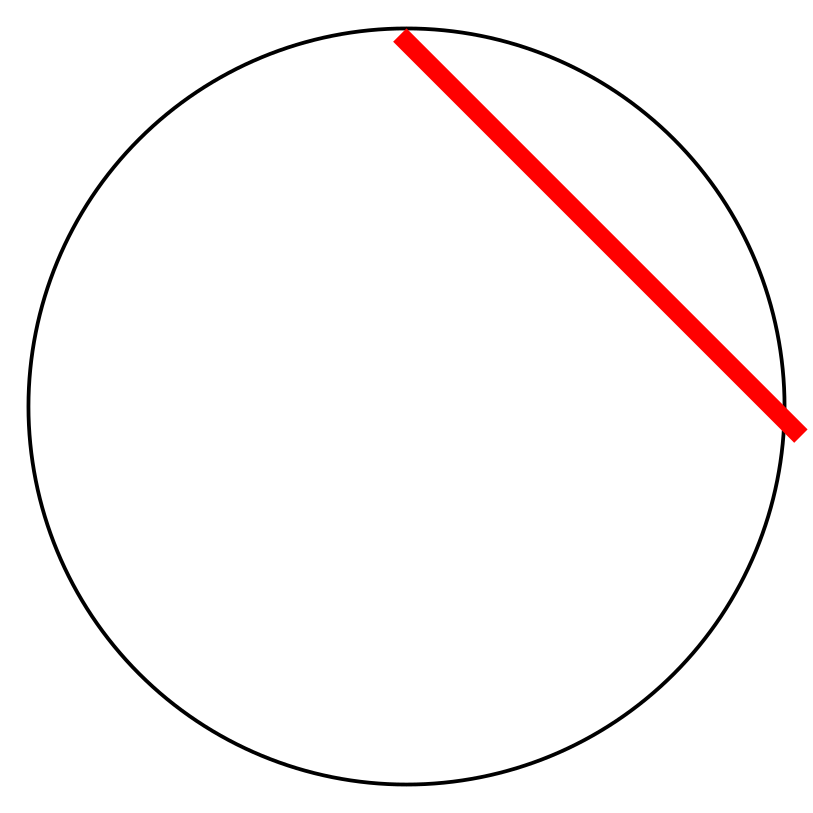
\includegraphics[width=0.49\textwidth]{spherical_approximations_line}
    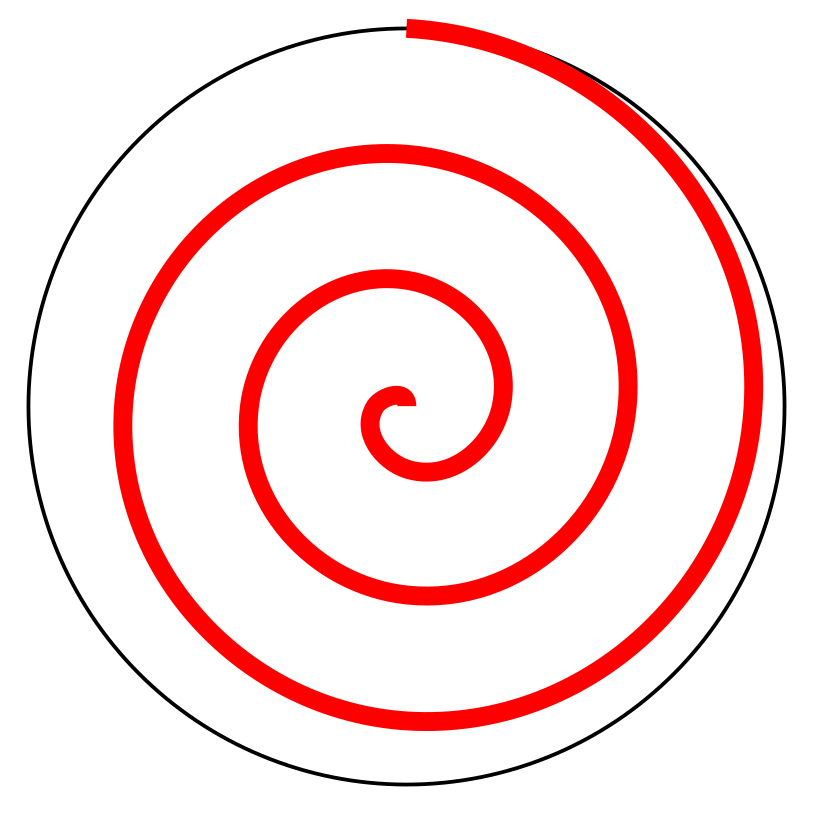
\includegraphics[width=0.49\textwidth]{spherical_approximations_spiral}
    \caption{Two possible interpretations of what a line with a constant angle in a spherical geometry could mean. On the left side a line with a constant angle (of 45 degrees) relative to the the surface where it started. Although this is the most intuitive way of interpreting a plate going down with a certain dip, when using very long plates this means that the plate may go back out the earth again. Note that this will only happen with unrealistically long slabs and/or dips very close to zero. On the right side is the other interpretation, constant dip with resprect to the surface directly above it. This resutls in a logarithmic sprial.}
    \label{fig:coordinate_systems_line_spiral}
\end{figure}

\begin{remark}
Note that currently only the constant angle relative to the surface where it started (the left side of figure \ref{fig:coordinate_systems_line_spiral}).
\end{remark}

The first option (line) is simpler, more intuitive and makes no assumptions about what a slab should do within the earth. The second option (spiral) is less intuitive, but implicitly includes gravity in the slab. Currently only the first option has been can be set through the \hl{depth method} parameter in the \hl{spherical} parameter, by setting the \hl{depth method} parameter to \hl{starting point}. Adding to the \WB{} file from the previous section by setting it to a spherical geometry, we get the following \WB{} file:

\begin{bashcode}{}
"version":0,
"coordinate system":{"spherical":{"depth method":"starting point"}},
"surface objects":{}
\end{bashcode}


\subsubsection{An endless world}
As you may have noticed, there are no bound give in the coordinate system of how far the model goes. So how does the \WB{} know how big your model is. The simple answer to this is that it doesn't. And that is because it doesn't need to know. Both in Cartesian and spherical coordinates, the world is endless, with a small note that in spherical coordinates, entering 361 degrees longitude will yield the same position as 1 degree longitude. This doesn't mean that they can always be use interchangeably. But we will explain more on that in section \ref{section:continetnal_plate}. For now it is important to know that the \WB{} world knows no limits.

\subsection{2d and 3d models}
The world we live in is an inherently 3d world, and so is the \WB{}. So no matter whether you are intending to use the \WB{} for a 2d or a 3d problem, you will need to define the 3d world. This doesn't mean that you can't use the \WB{} for 2d problems. On the contrary even, one of the core functionalities of the \WB{} are the 2d temperature and composition functions. The way this works is that you can define cross section through the 3d world. The cross section is given by providing the \hl{Cross section} parameter with two points on the surface. The first point will be the origin of the cross section, and the second point is the direction in which the cross section will be taken. Let's expand the Cartesian example from Listing \ref{lst:code_minimal_example_default_coordinate_system}, with a cross section:

\begin{bashcode}{An example showing how to use the cross section}
"version":0,
"cross section":[[100e3,100e3],[400e3,500e3]],
"coordinate system":{"cartesian":{}},
"surface objects":{}
\end{bashcode}

The first thing you will notice is a new notation: the square brackets \hl{[ ]}. These square brackets denote arrays. In this case it is an array, which contains two arrays, which each two points. An other way of putting it would be to say that it is an array of two 2d points. Remember from section \ref{section:coordinate_systems} that since we are using a Cartesian coordinate system, all the values have the unit meters. 
\\
A second thing to note is that we are only using 2d surface coordinates to define a plane in 3d space. The reason we can do this is that we already know what the range of the 3rth coordinate needs to be: from the bottom of the model to the surface. So there is no need to let the user specify this.
\\
When no cross section is given, the 3d functions of the \WB{} can be used with no problem. When you want to set up a 2d model, make sure you have provided the cross section parameter with the the correct surface coordinates.

\subsection{Plate tectonic features and models}
Before we can make our first real model, there is one more topic to discuss: features and models. As stated in the section on the idea behind the world builder (section \ref{section:idea_behind_WB}), we want users to be able to enter plate tectonic features and attach models to them to represent how certain properties, such as the temperature within that tectonic feature should be modeled. This is where the \hl{Surface object} parameter comes into play. Because through this parameter we can define the features and attach to them models for temperature and composition. In a generic way that looks something like this:

\begin{bashcode}{A example of a generic feature}
"version":0,
"surface objects":
{
  "feature name 1":
  {
    "temperature model":{"name":"none"},
    "composition model":{"name":"none"}
  }
}
\end{bashcode}

This is the very basics of what a feature is. It has a name and for every available property a model attached. Note that this example would not work in practice, because there is no feature implemented which is called \hl{Feature name 1}. Only specific feature names are allowed, which will be introduced from section \ref{section:continetnal_plate} and can be found in the the \WB{} input file parameter reference (see chapter \ref{chapter:WB_file_parameter_reference}).
\\
The property models in this case are set to \hl{none}. This is the only model which is always implemented for any property model. It does, as to be expected, nothing.
\\
A feature which does nothing is not very useful. So let's add an other feature in which we can actually see how parameters in a feature work.

\begin{bashcode}{A example of two generic features}
"version":0,
"surface objects":
{
  "feature name 1":
  {
    "temperature model":{"name":"none"},
    "composition model":{"name":"none"}
  },
                     
  "feature name 2":
  {
    "generic feature option 1":1000.0, 
    "generic feature option 2":"value 2",
    "temperature model":{"name":"temp. model name", "temp. parameter":100e3},
    "composition model":{"name":"comp. model name", "comp. parameter":1}
  }
}
\end{bashcode}

Here we have added a second feature (again a non-existent feature). The second feature now has parameters which are set, and even the temperature and composition models have parameters which can be set. Note that the features are separated by a comma. What is very important to know is that the order in which the features are listed matters. We haven't discussed the placing of features yet, but features may overlap, e.g. for one location, multiple features may be present. The list is read from top to bottom by the \WB{}, and every feature model receives the current value of the property in question. The specific model can then return a new value, which can be based on the value it received, but that doesn't have to be the case. 

\begin{remark}
The order in which the features are listed is important. It determines what happens when features overlap. In general it is a good rule to have the largest features at the top, and the smallest features at the bottom.
\end{remark}

This also means that there should be a starting value for each property. The starting value of the temperature is an adiabatic profile, of which the parameters global parameters of the \WB{} input file. All the compositions start out with a value of zero.

\subsection{Naming and placing the features in the world}
There are two feature parameters which are required for every feature. The first one is the parameter \hl{name}. This is required to make sure that the \WB{} files remain readable. The name should indicate what the feature represents in the real world, or at least in the model. 
\\
The second required parameter is the parameter is \hl{coordinates}. This is always an array of arrays of values, representing a list of 2d points on the surface. This list of 2d surface points can be interpreted by the features in two ways: an enclosed area or a line. How it is interpreted is documented by the individual feature. Here is our first generic example again, but now with the required parameters:

\begin{bashcode}{An example with a generic feature and the required parameters}
"version":0,
"surface objects":
{
  "feature name 1":
  {
    "name":"Eurasia",
    "coordinates":[[0,0],[0,100e3],[200e3,100e3],[200e3,0]],
    "generic feature option 1":1000.0, 
    "generic feature option 2":"value 2",
    "temperature model":{"name":"none"},
    "composition model":{"name":"none"}
  }
}
\end{bashcode}

\begin{remark}
Note that line features require at least two points and area features require at least three points.
\end{remark}

\section{The continental plate}
\label{section:continetnal_plate}
\subsection{A basic continental plate}
After all this theory, we can now finally start building a useful model. We begin with the continental plate, because this is probably the easiest feature there is to understand. It is a type of feature where the coordinates define an area on the surface of the world. It has not additional requirements, so a most basic continental plate \WB{} file looks like this:

\begin{bashcode}[label=lst:simple_continental_plate]{An example of the most basic continental plate}
"version":0,
"surface objects":
{
  "continental plate":
  {
    "name":"Eurasia",
    "coordinates":[[0,0],[0,100e3],[200e3,100e3],[200e3,0]],
    "temperature model":{"name":"none"},
    "composition model":{"name":"none"}
  }
}
\end{bashcode}

The example in listing \ref{lst:simple_continental_plate} still doesn't do anything yet. To make some interesting models we need to attach temperature and compositional models to it. For the continental feature there are different model available. The simplest model for both temperature and composition are the constant models. They set the temperature or a single compositions respectively to a specified value. In this case the only other thing they need to know is to which depth the continental plate goes. This is set by a the \hl{depth} paramater in each models.

\begin{bashcode}{A first functioning continental plate example}
"version":0,
"surface objects":
{
  "continental plate":
  {
    "name":"Eurasia",
    "coordinates":[[0,0],[0,100e3],[200e3,100e3],[200e3,0]],
    "temperature model":{"name":"constant", "depth"=100e3, "temperature"=293},
    "composition model":{"name":"constant", "depth"=20e3, "composition"=1}
  }
}
\end{bashcode}

This code should be pretty self-explanatory by now. It creates a continental plate which is a 100 km thick which has a temperature of 293 degree Kelvin and in the first 20 km the composition with number 1 is present. The value it is set to by default is 1.0, but this can be changed by using the \hl{value} parameter.
\subsection{linear temperature profile and layers}
Just having continents with a constant temperature and composition can be useful, but is not realistic. The next step we can take is by stating that a linear temperature gradient for a continental plate would be more realistic. To achieve a linear gradient we will need to change the temperature model to the \hl{linear} temperature model. This temperature model has two required parameter and one optional. The two required parameters are the \hl{depth} and the \hl{top temperature}. The \hl{bottom temperature} is an optional which is not provided, the adiabatic temperature at the depth of the bottom of the temperature part of the continental plate is used. In this case that is what we want, so we will leave out the \hl{bottom temperature}.

\begin{bashcode}{Using the linear temperature model}
"version":0,
"surface objects":
{
  "continental plate":
  {
    "name":"Eurasia",
    "coordinates":[[0,0],[0,100e3],[200e3,100e3],[200e3,0]],
    "temperature model":{"name":"linear", "depth"=100e3, "top temperature"=293},
    "composition model":{"name":"constant", "depth"=20e3, "composition"=1}
  }
}
\end{bashcode}

We can also improve the compositional representation through a composition model called \hl{constant layers}. This allows us to for example have a separate composition for the upper crust, lower crust and the rest of the plate. This is represented by an array of layer objects. These layer objects each have a composition and a thickness:

\begin{bashcode}{Using the linear temperature model}
"version":0,
"surface objects":
{
  "continental plate":
  {
    "name":"Eurasia",
    "coordinates":[[0,0],[0,100e3],[200e3,100e3],[200e3,0]],
    "temperature model":{"name":"linear", "depth"=100e3, "top temperature"=293},
    "composition model":
    {
      "name":"constant", "depth"=20e3, 
      "layers":[{"composition":0, "thickness":20e3},
                 {"composition":1, "thickness":30e3},
                 {"composition":2, "thickness":50e3}]
      }
  }
}
\end{bashcode}

Like the feature list, the order is important. The first layer is the top layer, which reaches to a depth of 20 km. The second layer starts from 20 km and with a thickness of 30 km it reaches to 50 km. 

\begin{remark}
Note that any layer beyond the continental plate depth is ignored. So in this case if we made the third layer 100 km thick, the results would still be the same.
\end{remark}

With this you are now able to create your own continents. Congratulations and well done for reaching this point in the manual! Next up are Oceanic plates.

\section{The oceanic plate}
Now that you understand continental plates, oceanic plates will be easy to understand. And if you will look closely in the parameter reference, the oceanic plate has all the models which the continental plate also currently has. The difference is that the oceanic plate has currently one more temperature model, which the continental plate doesn't have, and wouldn't make sense to have. This is the \hl{plate model}. This name may sound confusing, since we have been talking about plates all the time. The reason we use this name is that this is the name commonly used in the geodynamics community, see for example \cite{fowler2005}. 
\\
This temperature model takes exactly the same parameters as the linear temperature model, but as two more parameters. The first one is is the \hl{spreading velocity} in meters per second (TODO: figure out if it is full or half spreading rate). The secon one is a list of 2d points where the ridge is located. From the ridge defined by these points, the plate will cool.

\begin{bashcode}{Using the oceanic plate's "plate model" temperature model}
"version":0,
"surface objects":
{
  "oceanic plate":
  {
    "name":"Atlantic",
    "coordinates":[[0,0],[0,100e3],[200e3,100e3],[200e3,0]],
    "temperature model":
    {
      "name":"linear", "depth"=100e3, "top temperature"=293,
      "plate velocity":0.01", ridge points":[[50e3,0],[50e3,50e3],[100e3,100e3]]
    },
    "composition model":{"name":"constant", "depth"=20e3, "composition"=1}
  }
}
\end{bashcode}

\section{The subducting plate}
While the continental plate and the oceanic plate are both area features, we now come across the first line feature: the subducting plate. This means that the coordinates defined in this feature do not form an area on the surface, which we extrapolate into the depth, but instead it represents the intersection between the plane and the surface. Beside the two normal required parameters, this feature requires at least two more parameters to be specified. The first one is called the \hl{reference point}. In simple terms, a subducting plate, with a angle between 0 and 90 degrees, will always point in the direction of the location of this reference point. The second parameter is the called \hl{segments}. The way this parameter works is best explained by an example. Let's make for our first slab a slab which goes down with an angle of 45 degrees, is 200 km long and 100 km thick.

\begin{bashcode}{Using the oceanic plate's "plate model" temperature model}
"version":0,
"surface objects":
{
  "subducting plate":
  {
    "name":"Lesser Antilles slab", "reference point"=[0,0]
    "coordinates":[[0,0],[50e3,50e3],[200e3,100e3]],
    "segments":
    {
      "all":[{"length":200e3, "thickness":[100e3], "angle":[45]}]
    }
    "temperature model":{"name":"none"},
    "composition model":{"name":"none"}
  }
}
\end{bashcode}

As can be seen from this example, the actual plate segment is encapsulated by a parameter named \hl{all}. For now ignore this an focus on the segment itself. It has exactly the parameter we want to have: length, thickness and angle. But as you may notice, thickness and angle are written as single values in an array. This is because these values can actually change over the length of the slab segment. As an example, let's now make a segment which is still 200 km long, but start with a thickness of 100 km, but end with a thickness of 50 km. Futhermore, lets start with an angle of 0 degrees and end with 45 degrees. Also let's add a second segment which is a 100 km long, 50 km thick in the beginning and 100 km thick in the end and has an angle which goes from 45 to zero degrees. The input file then should look like this:

\begin{bashcode}{Using the oceanic plate's "plate model" temperature model}
"version":0,
"surface objects":
{
  "subducting plate":
  {
    "name":"Lesser Antilles slab", "reference point"=[0,0]
    "coordinates":[[0,0],[50e3,50e3],[200e3,100e3]],
    "segments":
    {
      "all":[{"length":200e3, "thickness":[100e3,50e3], "angle":[0,45]},
              {"length":100e3, "thickness":[50e3,100e3], "angle":[45,0]}]
    }
    "temperature model":{"name":"none"},
    "composition model":{"name":"none"}
  }
}
\end{bashcode}

This already makes it possible to create quite complex and realistic slab geometries, but there is still one step to take. Real world slab do not only change in depth, but can also change laterally, i.e. between the coordinates given for the feature. Internally each of the coordinates gets a number, starting from zero. So if we want to overwrite the segment angle at point [50e3,50e3], and set it there to 60, we can do the following:

\begin{bashcode}{Using the oceanic plate's "plate model" temperature model}
"version":0,
"surface objects":
{
  "subducting plate":
  {
    "name":"Lesser Antilles slab", "reference point"=[0,0]
    "coordinates":[[0,0],[50e3,50e3],[200e3,100e3]],
    "segments":
    {
      "all":[{"length":200e3, "thickness":[100e3,50e3], "angle":[0,45]},
              {"length":100e3, "thickness":[50e3,100e3], "angle":[45,0]}]
      "1":[{"length":200e3, "thickness":[100e3,50e3], "angle":[60]},
             {"length":100e3, "thickness":[50e3,100e3], "angle":[60]}]
    }
    "temperature model":{"name":"none"},
    "composition model":{"name":"none"}
  }
}
\end{bashcode}

Between the coordinates 0 and 1 and 1 and 2 the \WB{} will interpolate the angle. The same trick works for the length and thickness. With the help of this functionality, the  geometry of the slabs are extremely costumizable. But having complex slab geometries without attaching a temperature or compositional model is not much use. Like the continental plate, this feature supports the constant temperature and compositional modules, and the layer compositional module. Only the linear temperature is missing, although this one might be in before the release of version 0.1.0 of the \GWB{}. The models use instead of the depth the distance from the top of the slab geometry to define the composition or temperature. A unique temperature model for this feature is called the \hl{plate model}, and implements the McKenzie (1970) temperature model for a slab which enters the mantle (see \cite{mckenzie1970}). The only two parameter which are required for this model are a reference \hl{density} and the \hl{plate velocity}.

\begin{bashcode}{Using the oceanic plate's "plate model" temperature model}
"version":0,
"surface objects":
{
  "subducting plate":
  {
    "name":"Lesser Antilles slab", "reference point"=[0,0]
    "coordinates":[[0,0],[50e3,50e3],[200e3,100e3]],
    "segments":
    {
      "all":[{"length":200e3, "thickness":[100e3,50e3], "angle":[0,45]},
              {"length":100e3, "thickness":[50e3,100e3], "angle":[45,0]}]
      "1":[{"length":200e3, "thickness":[100e3,50e3], "angle":[60]},
             {"length":100e3, "thickness":[50e3,100e3], "angle":[60]}]
    }
    "temperature model":{"name":"plate model", "density":3300e3, 
                           "plate velocity":0.01},
    "composition model":{"name":"constant", "depth"=20e3, "composition"=1}
  }
}
\end{bashcode}
\section{Final comments}
There you have it, all the basics of the \GWB{}! You have seen how each component of the \WB{} works, and how the ideas are implemented. But in the end the best way to learn and to find out what the \WB{} is really capable of is to just try it out. If stumble on a problem or think that something should work differently or even that you really need a specific functionality, don't stay silent. Please let it know on github: \url{https://github.com/GeodynamicWorldBuilder/WorldBuilder}. Feel free to make an issue, so that your problem or idea can be discussed. 
\\
We are also happy if you want to contribute code or documentation. If you find a mistake in the manual or code, even is it is a simple spelling or grammatical mistake, please report it. The effort is really appreciated. It would also make for a great first pull request!
\chapter{\WB{} file parameter reference}
\label{chapter:WB_file_parameter_reference}
\section{Global parameters}
\begin{parameterbox}{version}{true}{unsigned int}{NaN::ISNAN}
The major version number for which the input file was written.
\end{parameterbox}
%\begin{parameterbox}{coordinate system}{false}{string}{cartesian}
%This determines the coordinate system. The choices are "Cartesian" and "spherical".
%\end{parameterbox}
\begin{parameterbox}{potential mantle temperature}{false}{double}{1600}
The potential temperature of the mantle at the surface in Kelvin.
\end{parameterbox}
\begin{parameterbox}{surface temperature}{false}{double}{293.15}
The temperature at the surface in Kelvin.
\end{parameterbox}
\begin{parameterbox}{thermal expansion coefficient}{false}{double}{3.5e-5}
The thermal expansion coefficient in $K^{-1}$.
\end{parameterbox}
\begin{parameterbox}{specific heat}{false}{double}{1250}
The specific heat Cp in $J kg^{-1} K^{-1}$.
\end{parameterbox}
\begin{parameterbox}{thermal diffusivity}{false}{double}{0.804e-6}
Set the thermal diffusivity in $m^{2} s^{-1}$.
\end{parameterbox}
\begin{parameterbox}{surface rotation angle}{false}{double}{0}
The angle with which the model should be rotated around the surface rotation point. Note not implemented.
\end{parameterbox}
\begin{parameterbox}{surface rotation point}{false}{Point<2>}{[0,0]}
The point where should be rotated around.
\end{parameterbox}
\section{coordinate systems}
\subsection{cartesian}
\subsection{spherical}
\begin{parameterbox}{depth method}{true}{String}{}
The method used to go with an angle into depth in the case of spherical coordinates.
\end{parameterbox}

%%%%%%%%%%%%%%%%%%%%%%%%%%%%%%%%%%%%%%%%%%%%%%%%%%%%%%%%%%%%%%%%%%%%%%%%%%%%
%%%%%%%%%%%%%%%%%%%%%%%%%%%%%%%%% Features %%%%%%%%%%%%%%%%%%%%%%%%%%%%%%%%% 
%%%%%%%%%%%%%%%%%%%%%%%%%%%%%%%%%%%%%%%%%%%%%%%%%%%%%%%%%%%%%%%%%%%%%%%%%%%%
\section{features}

%%%%%%%%%%%%%%%%%%%%%%%%%%%%%%%%%%%%%%%%%%%
%%%%%%%%%%%% Continental plate %%%%%%%%%%%% 
%%%%%%%%%%%%%%%%%%%%%%%%%%%%%%%%%%%%%%%%%%%
\subsection{The continental plate}
\begin{parameterbox}{name}{true}{String}{}
The name which the user has given to the feature.
\end{parameterbox}

\begin{parameterbox}{coordinates}{true}{Array of Points<2>}{}
An array of Points representing an array of coordinates where the feature is located. This is an area feature.
\end{parameterbox}

%%%%%%%%%%%% temperature model %%%%%%%%%%%% 
\subsubsection{temperature model}
\begin{parameterbox}{name}{true}{String}{}
The name of the temperature model.
\end{parameterbox}

%%%%% Constant
\paragraph{constant}
\begin{parameterbox}{depth}{true}{Double}{}
The depth in meters to which the temperature of this feature is present.
\end{parameterbox}

\begin{parameterbox}{temperature}{true}{Double}{}
The temperature in degree Kelvin which this feature should have
\end{parameterbox}

%%%%% Linear
\paragraph{linear}
\begin{parameterbox}{depth}{true}{Double}{}
The depth in meters to which the temperature rises (or lowers) to.
\end{parameterbox}

\begin{parameterbox}{top temperature}{false}{Double}{293.15}
The temperature in degree Kelvin at the top of this block.
\end{parameterbox}

\begin{parameterbox}{bottom temperature}{false}{Double}{}
The temperature in degree Kelvin a the bottom of this block. If this value is not defined, the adiabatic temperature at this depth is used.
\end{parameterbox}

%%%%%%%%%%%% composition model %%%%%%%%%%%%
\subsubsection{composition model}
\begin{parameterbox}{name}{true}{String}{}
The name of the composition model.
\end{parameterbox}

%%%%% Constant
\paragraph{constant}
\begin{parameterbox}{depth}{true}{Double}{}
The depth in meters to which the composition of this feature is present.
\end{parameterbox}

\begin{parameterbox}{composition}{false}{Unsigned int}{1.0}
The number of the composition that is present there.
\end{parameterbox}

\begin{parameterbox}{value}{false}{Double}{}
The value between 0 and 1 of how much this composition is present.
\end{parameterbox}

%%%%% Constant Layers
\paragraph{constant layers}
\begin{parameterbox}{layers}{true}{Array of Layers}{}
A list of layers with a certain composition and thickness.
\end{parameterbox}

\begin{parameterbox}{composition}{false}{Unsigned int}{}
The number of the composition that is present there.
\end{parameterbox}

\begin{parameterbox}{value}{false}{Double}{}
The value between 0 and 1 of how much this composition is present.
\end{parameterbox}

%%%%%%%%%%%%%%%%%%%%%%%%%%%%%%%%%%%%%%%%%%%
%%%%%%%%%%%%%% Oceanic plate %%%%%%%%%%%%%% 
%%%%%%%%%%%%%%%%%%%%%%%%%%%%%%%%%%%%%%%%%%%
\subsection{oceanic plate}
\begin{parameterbox}{name}{true}{String}{}
The name which the user has given to the feature.
\end{parameterbox}

\begin{parameterbox}{coordinates}{true}{Array of Points<2>}{}
An array of Points representing an array of coordinates where the feature is located. This is an area feature.
\end{parameterbox}

%%%%%%%%%%%% temperature model %%%%%%%%%%%% 
\subsubsection{temperature model}
\begin{parameterbox}{name}{true}{String}{}
The name of the temperature model.
\end{parameterbox}

%%%%% Constant
\paragraph{constant}
\begin{parameterbox}{depth}{true}{Double}{}
The depth in meters to which the temperature of this feature is present.
\end{parameterbox}

\begin{parameterbox}{temperature}{true}{Double}{}
The temperature in degree Kelvin which this feature should have
\end{parameterbox}

%%%%% Linear
\paragraph{linear}
\begin{parameterbox}{depth}{true}{Double}{}
The depth in meters to which the temperature rises (or lowers) to.
\end{parameterbox}

\begin{parameterbox}{top temperature}{false}{Double}{293.15}
The temperature in degree Kelvin at the top of this block.
\end{parameterbox}

\begin{parameterbox}{bottom temperature}{false}{Double}{}
The temperature in degree Kelvin a the bottom of this block. If this value is not defined, the adiabatic temperature at this depth is used.
\end{parameterbox}


%%%%% plate model
\paragraph{plate model}
\begin{parameterbox}{depth}{true}{Double}{}
The depth in meters to which the temperature rises (or lowers) to.
\end{parameterbox}

\begin{parameterbox}{top temperature}{false}{Double}{293.15}
The temperature in degree Kelvin at the top of this block.
\end{parameterbox}

\begin{parameterbox}{bottom temperature}{false}{Double}{}
The temperature in degree Kelvin a the bottom of this block. If this value is not defined, the adiabatic temperature at this depth is used.
\end{parameterbox}

\begin{parameterbox}{spreading velocity}{true}{Double}{}
The spreading velocity of the plate in meter per year. This is the velocity with which one side moves away from the ridge.
\end{parameterbox}

\begin{parameterbox}{ridge points}{true}{Array of Point<2>}{}
A list of 2d points which define the location of the ridge.
\end{parameterbox}

%%%%%%%%%%%% composition model %%%%%%%%%%%%
\subsubsection{composition model}
\begin{parameterbox}{name}{true}{String}{}
The name of the composition model.
\end{parameterbox}

%%%%% Constant
\paragraph{constant}
\begin{parameterbox}{depth}{true}{Double}{}
The depth in meters to which the composition of this feature is present.
\end{parameterbox}

\begin{parameterbox}{composition}{false}{Unsigned int}{1.0}
The number of the composition that is present there.
\end{parameterbox}

\begin{parameterbox}{value}{false}{Double}{}
The value between 0 and 1 of how much this composition is present.
\end{parameterbox}

%%%%% Constant Layers
\paragraph{constant layers}
\begin{parameterbox}{layers}{true}{Array of Layers}{}
A list of layers with a certain composition and thickness.
\end{parameterbox}

\begin{parameterbox}{composition}{false}{Unsigned int}{}
The number of the composition that is present there.
\end{parameterbox}

\begin{parameterbox}{value}{false}{Double}{}
The value between 0 and 1 of how much this composition is present.
\end{parameterbox}


%%%%%%%%%%%%%%%%%%%%%%%%%%%%%%%%%%%%%%%%%%%
%%%%%%%%%%%%% Subducting plate %%%%%%%%%%%% 
%%%%%%%%%%%%%%%%%%%%%%%%%%%%%%%%%%%%%%%%%%%
\subsection{The subducting plate}
\begin{parameterbox}{name}{true}{String}{}
The name which the user has given to the feature.
\end{parameterbox}

\begin{parameterbox}{coordinates}{true}{Array of Points<2>}{}
An array of Points representing an array of coordinates where the feature is located. This is a line feature.
\end{parameterbox}

%%%%%%%%%%%% temperature model %%%%%%%%%%%% 
\subsubsection{temperature model}
\begin{parameterbox}{name}{true}{String}{}
The name of the temperature model.
\end{parameterbox}

%%%%% Constant
\paragraph{constant}
\begin{parameterbox}{depth}{true}{Double}{}
The depth in meters to which the temperature of this feature is present.
\end{parameterbox}

\begin{parameterbox}{temperature}{true}{Double}{}
The temperature in degree Kelvin which this feature should have
\end{parameterbox}

%%%%% plate model
\paragraph{plate model}
\begin{parameterbox}{density}{true}{Double}{}
The reference density of the subducting plate.
\end{parameterbox}

\begin{parameterbox}{plate velocity}{false}{Double}{}
The velocity in meters per year with which the plate subducts.
\end{parameterbox}

\begin{parameterbox}{thermal conductivity}{false}{Double}{2.0}
The thermal conductivity of the subducting plate material in $W m^{-1} K^{-1}$.
\end{parameterbox}

\begin{parameterbox}{thermal expansion coefficient}{false}{Double}{3.5e-5}
The thermal expansivity of the subducting plate material in $K^{-1}$.
\end{parameterbox}

\begin{parameterbox}{specific heat}{true}{Array of Point<2>}{1250}
The specific heat of the subducting plate material in $J kg^{-1} K^{-1}$.
\end{parameterbox}

%%%%%%%%%%%% composition model %%%%%%%%%%%%
\subsubsection{composition model}
\begin{parameterbox}{name}{true}{String}{}
The name of the composition model.
\end{parameterbox}

%%%%% Constant
\paragraph{constant}
\begin{parameterbox}{depth}{true}{Double}{}
The depth in meters to which the composition of this feature is present.
\end{parameterbox}

\begin{parameterbox}{composition}{false}{Unsigned int}{1.0}
The number of the composition that is present there.
\end{parameterbox}

\begin{parameterbox}{value}{false}{Double}{}
The value between 0 and 1 of how much this composition is present.
\end{parameterbox}

%%%%% Constant Layers
\paragraph{constant layers}
\begin{parameterbox}{layers}{true}{Array of Layers}{}
A list of layers with a certain composition and thickness.
\end{parameterbox}

\begin{parameterbox}{composition}{false}{Unsigned int}{}
The number of the composition that is present there.
\end{parameterbox}

\begin{parameterbox}{value}{false}{Double}{}
The value between 0 and 1 of how much this composition is present.
\end{parameterbox}

\part{Information for developing for the World Builder}
\chapter{Introduction}
\section{prerequisites}
To contribute to the world builder there the only prerequisites is that you are willing to contriube to open-source software under the GNU LESSER GENERAL PUBLIC LICENSE version 2.1. See the licence document in the repository for more information. As mentioned in part 1 of the manual, we really appreciate any contribution!
\\
If you want to contribute code, some knowledge of of c++ is required. For writing and changing plugins, a basic knowledge of how variables, loops and functions work should be sufficient to be able to contribute. 
\\
As a version management system, and also as a system to manage and discuss contributions, we use git and github. Some basic knowledge on how git works will speed up how fast you can contribute to the \WB{}.
\\
If there is something you do not understand, do not hesitate to ask a question by making a issue on github.

\section{Conventions}
There are several conversions used when writing code. Because the code is still very young, we will only name the most important ones. 
\begin{enumerate}
    \item all parameters in the \WB{} parameter file are lower case.
    \item all variable names are snake case (variable\_name).
    \item all function names are snake case (function\_name).
    \item all class names are camel case (ClassName).
\end{enumerate}
\chapter{Structure of the code}
Currently the code is changing to rapidly for it to be useful to write this section.
\chapter*{Bibliography}
\printbibliography[heading=bibempty]
\addcontentsline{toc}{chapter}{\textcolor{ocre}{Bibliography}}
\end{document}
